
Принципиальная схема:
\begin{center}
        \begin{figure}[h!]
                \center{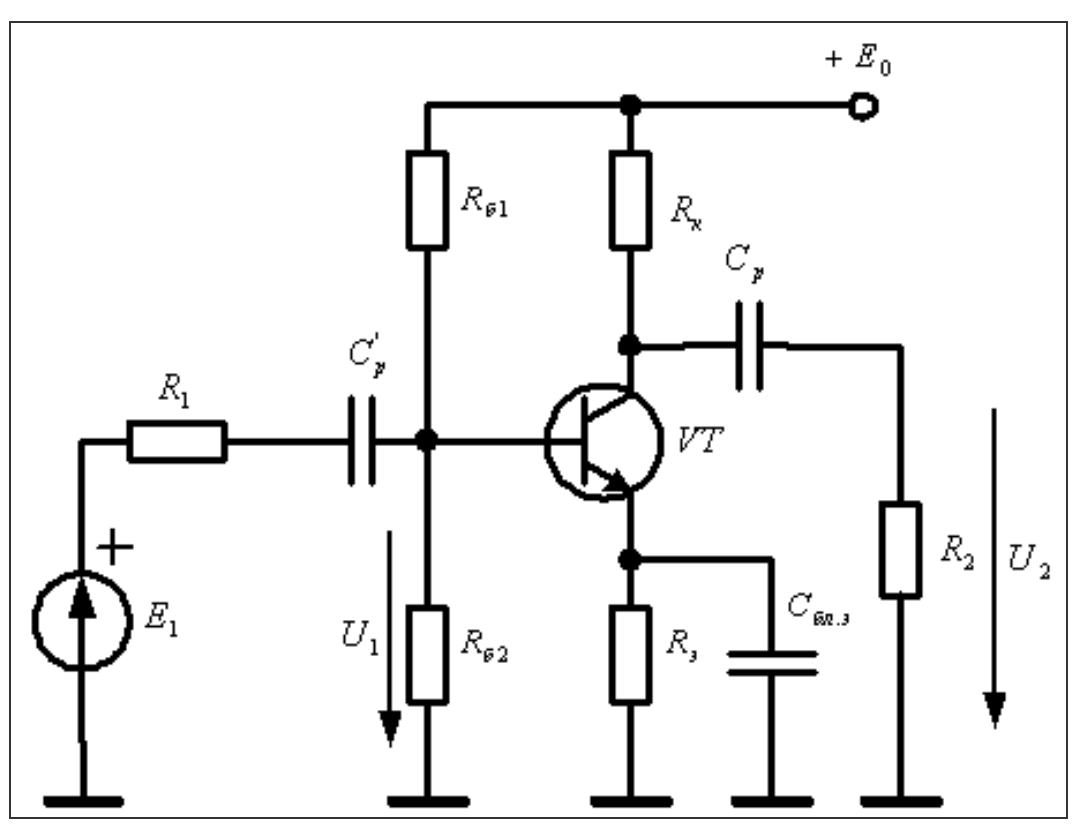
\includegraphics[scale=0.2]{oe.png}}
                \caption{Какой из трех каскадов ОЭ, ОБ,ОК и при каких условиях будет иметь по отношению к другим самую большую верхнюю граничную частоту}
        \end{figure}
\end{center}


Верхняя граничная частота каскада - частот полосы пропускания
$f_B = 1/(2\pi*\tau_B)$		(*)
На этой частоте Uвых в $\surd(2)$ раз меньше, чем на средней частоте. На средней частоте можно не учитывать частотную зависимость коэффициента передачи по току и емкость Cкэ - барьерную емкость коллекторного перехода.

Верхняя граничная частота каскада зависи от параметров транзисторов: B, Ск, rb, Rн, Cн, Rг и схемы включения транзистора.

В (*) $\tau_B = G(\tau_B) + C_\textit{кэ}R_\textit{КН})+R_\textit{КН}+C_\textit{Н}$
$\tau_B$ - время жизни носителей заряда в базе
$\tau_B = 1/(2\pi*f_B)$	

ЗДЕСЬ НАДО ВСТАВИТЬ РИСУНОК pict11_1.png


$C_\textit{кэ} = C_\textit{к}*B$ - барьерная емкость КП

$C_\textit{кэ} = C_\textit{кб}*(B+1)$

G-коэффициент токораспределения. Зависит от того, сколько носителей заряда пойдет во входную цепь.
Доля пропавшх носителей выражается как $\tau_\alpha/\tau_\beta$ , где $\tau_\alpha/$ - время пролета, а $\tau_\beta$ - время жизни.

Для  того чтобы сравнить верхние граничные частоты каскадов ОЭ, ОБ,ОК достаточно рассмотреть соответствующие G при равных условиях, при этом чем меньше G, тем лучше.

Рассмотрим каскад ОЭ.
Этот и все каскады далее расматриватся на СЧ, где влияние емкостей несущественно.
\begin{center}
        \begin{figure}[h!]
                \center{\includegraphics[scale=0.9]{eoe.png}}
                \caption{эквивалентная схема с ОЭ}
                \label{EOE}
        \end{figure}
\end{center}

$G_\textit{OE} = ([R_g ||(R_1||R_2)] + r_b+r_e)/([R_g ||(R_1||R_2)] + r_b+r_e(B+1))$
Где в числителе - полное сопротивление усилителя при НЧ, а в знаменателе слагаемое с (В+1) - отражает утерю усилителем коэффициента усиления по току.

Если Rг||(R1||R2) = 0, а rб мало, то $G_\textit{OE} =1/(B+1)$
Если Rг||(R1||R2) -> $\infty$, а rб мало, то $G_\textit{OE} \longrightarrow 1$


Рассмотрим каскад ОБ.

\begin{center}
        \begin{figure}[h!]
                \center{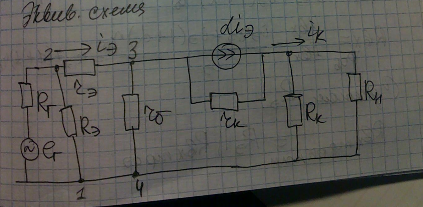
\includegraphics[scale=0.9]{eob.png}}
                \caption{эквивалентная схема с ОБ}
                \label{EOB}
        \end{figure}
\end{center}

$G_\textit{OB} = ([R_g ||(R_1||R_2)] + r_b+r_e)/((B+1)*[R_g ||(R_1||R_2)] + r_b+r_e(B+1))$

$(B+1)*[R_g ||(R_1||R_2)]$ - определяется тем,что входной ток - эмиттерный

Если Rг||(R1||R2) = 0, а rб мало, то $G_\textit{OB}=G_\textit{OE} =1/(B+1)$
Если Rг||(R1||R2) -> $\infty$, а rб мало, то $G_\textit{OE} \longrightarrow 1/(B+1)$

Рассмотрим каскад ОК.

\begin{center}
        \begin{figure}[h!]
                \center{\includegraphics[scale=0.9]{ok1.png}}
                \caption{эквивалентная схема с ОК}
                \label{OK1}
        \end{figure}
\end{center}

$G_\textit{OB} = ([R_g ||(R_1||R_2)] + r_b+r_e+R_\textit{эн})/([R_g ||(R_1||R_2)] + r_b+r_e(B+1) + R_\textit{эн}(B+1)) = ([R_g ||(R_1||R_2)] + r_b+r_e+R_\textit{эн})/([R_g ||(R_1||R_2)] + (r_b+r_e+R_\textit{эн})*(B+1))$

Если Rг||(R1||R2) = 0, а rб мало, то $G_\textit{OB}=G_\textit{OE} =1/(B+1)$
Если Rг||(R1||R2) -> $\infty$, а rб мало, то $G_\textit{OE} \longrightarrow 1)$

ТУТ НАДО ВСТАВИТЬ ТАБЛИЦУ КАК НА ФОТКЕ tbl13_1.png

